\section{ConvR: Adaptive Convolution for Multi-Relational Learning}
\subsection{研究背景与目的}

\begin{frame}[c]{Introduction}

\begin{block}{Adaptive Convolution for Multi-Relational Learning}
	\begin{itemize}
	    \item Author: Xiaotian Jiang, Quan Wang, Bin Wang.
	    \item Lab: Cloud and Smart Industries Group, Tencent. Baidu Inc. Xiaomi AI Lab.
	    \item Comments: NAACL 2019.
	\end{itemize}
\end{block}

\begin{block}{Abstract}
	\begin{itemize}
	    \item 基于卷积神经网络的模型能学习更丰富、更具表象力的Embedding,作者将它应用在了知识图谱的关系预测任务中。
	    \item 过去的卷积设计方式未能完全捕捉实体和关系之间完整的交互关系,作者重新设计了一种自适应卷积方式,能最大化实体与关系的交互,称作ConvR。
	    \item ConvR实验效果在多个数据集的效果和效率指标上均优于各Baseline。
	\end{itemize}
\end{block}

\end{frame}

\subsection{研究内容与方法}

\begin{frame}[c]{Background}

\begin{itemize}
    \item 知识图谱可以表示为$G=(E,R)$,其中$E$和$R$分别表示实体(节点)集合和关系(边)集合。对于知识图谱里的三元组$(h,r,t)$可以表示为两个实体节点$h$和$t\ (h, t \in E)$之间存在类型为$r\ (r\in R)$的边。\\ 
    \begin{center}
        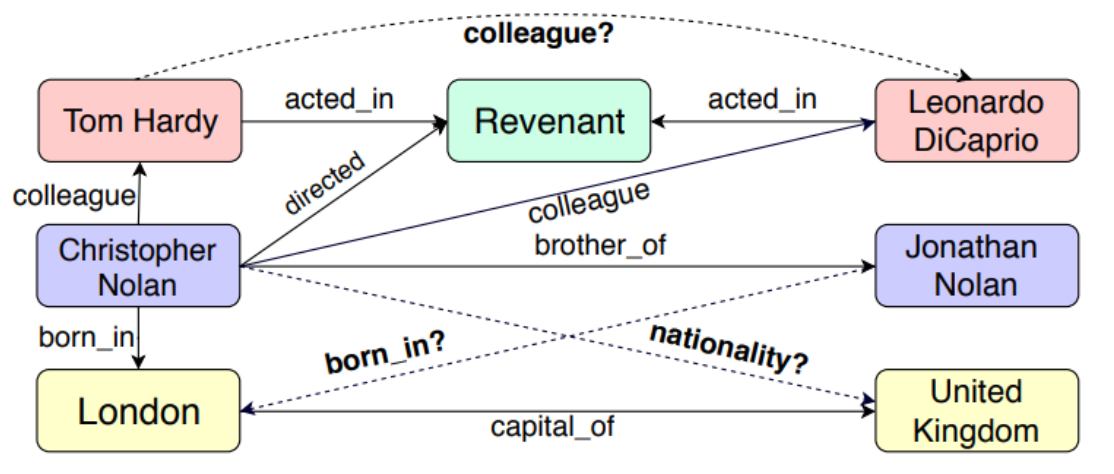
\includegraphics[width=8cm]{assets/1.png}
    \end{center}
    \item 表示学习模型:学习实体和关系的有效嵌入表示(Embedding),服务于下游任务。
    \item 关系预测模型:学习评分函数$f(\cdot)$,输入待预测三元组$(h,r,t)$,输出关于它的评分$f(h,r,t)$。评分规则取决于损失函数的设计。例如\texttt{MarginLoss}约束真实三元组分数要比负采样的虚假三元组分数高。
\end{itemize}

\end{frame}

\begin{frame}[c]{ConvE - Review}

\begin{itemize}
    \item 将关系Embedding和实体Embedding重塑成2D向量,堆叠成一个新的2D向量,使用$3\times 3$的卷积核进行卷积。\\
    \begin{center}
        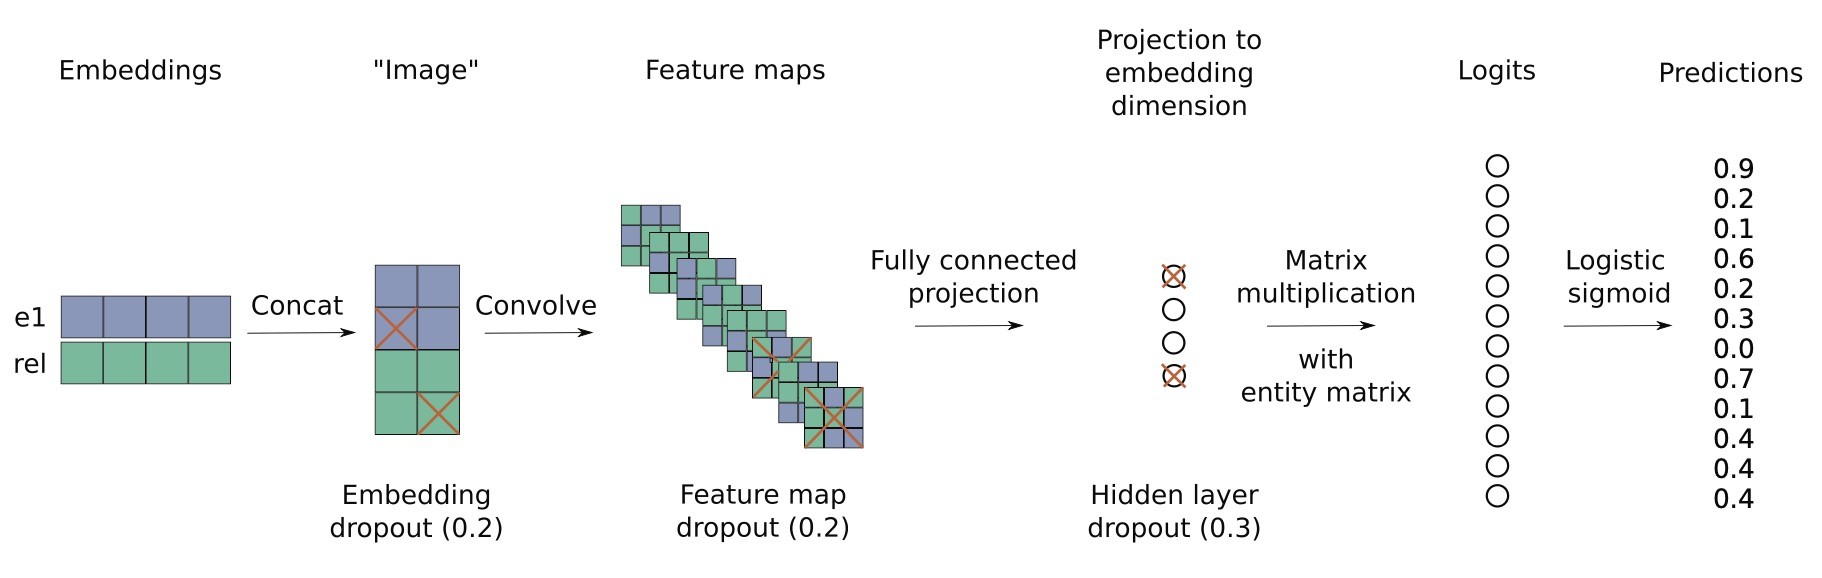
\includegraphics[width=10cm]{assets/2.png}
    \end{center}
    \item ConvE作者认为二维卷积可以捕捉更多实体和关系的特征交互信息。
    \item 损失函数使用\texttt{BCELoss},即$\mathcal{L}(h,r)=-\frac{1}{|\mathcal{E}|}\sum\limits_{t\in \mathcal{E}}y_{t}^{h,r}\log(p_{t}^{h,r})+(1-y_{t}^{h,r})\log(1-p_{t}^{h,r})$,其中$y_{t}^{h,r}$是三元组$(h,r,t)$的标签,$p_{t}^{h,r}$是模型对三元组的评分预测。损失函数的约束让真实的三元组评分趋近于$1$,负采样的虚假三元组评分趋近于$0$。
    \item 但ConvR作者认为这种使用堆叠的方式来进行卷积不够充分。
\end{itemize}

\end{frame}

\begin{frame}[c]{ConvR - Architecture}
    
\begin{itemize}
    \item ConvE中使用的卷积器是若干个$3\times 3$的可训练的卷积核(Global filters),而ConvR则使用关系的Embedding代替ConvE里这个卷积器来对实体Embedding进行卷积。\\
    \begin{center}
        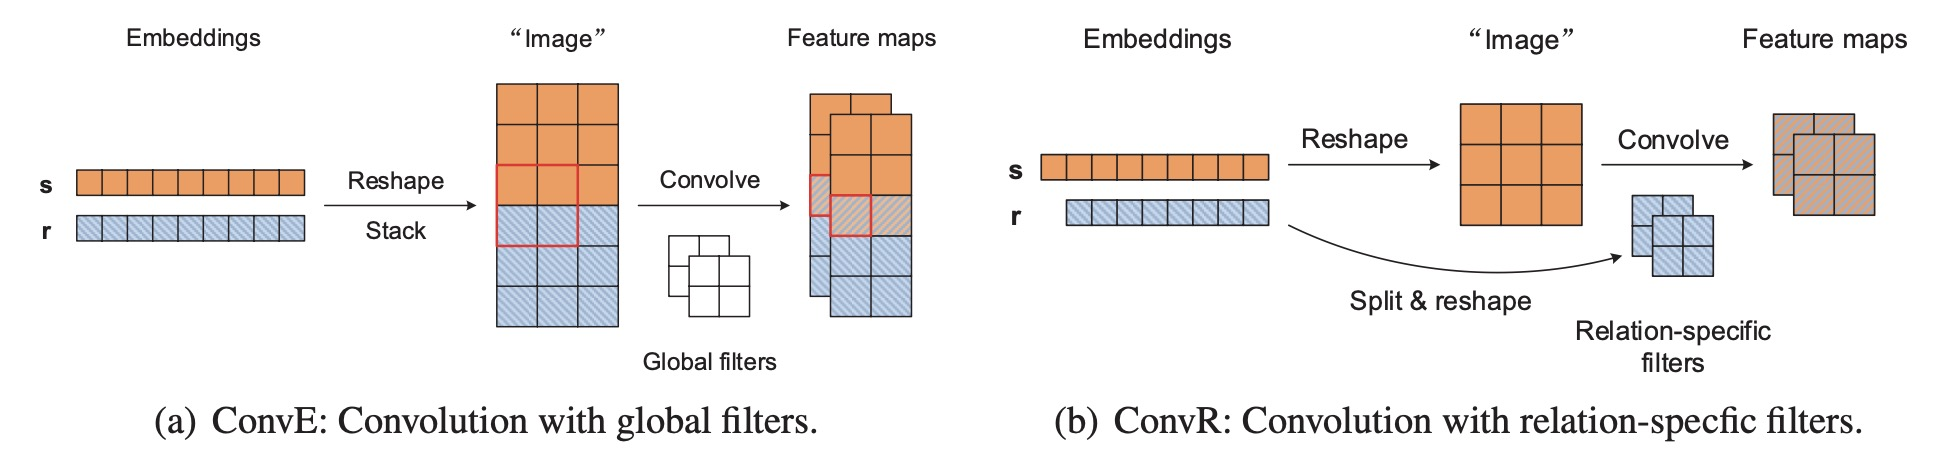
\includegraphics[width=12cm]{assets/3.png}
    \end{center}
    \item 直观感受——不需要训练额外的卷积核作为网络参数(参数变少);卷积时候输入的2D向量缩小了一倍(由原来的实体和关系重塑并拼接变成只需要输入实体的重塑向量,训练速度变快)。
\end{itemize}
    
\end{frame}

\begin{frame}[c]{ConvR - Details}

\begin{itemize}
    \item 将关系向量R的Embedding划分为若干块,即$\bm{r}\in \mathbb{R}^{d_r}\to \bm{r}=\{r^{(i)}\in \mathbb{R}^{h\times w}\}$。每一块单独作为一个独立的卷积核去和头实体的Embedding进行卷积得到对应的Feature map,即$\bm{h}\in \mathbb{R}^{d_e^h\times d_e^w} \to \bm{c}=\{c^{(i)}\in \mathbb{R}^{(d_e^h-h+1)\times (d_e^w-w+1)}\}$。\\
    \begin{center}
        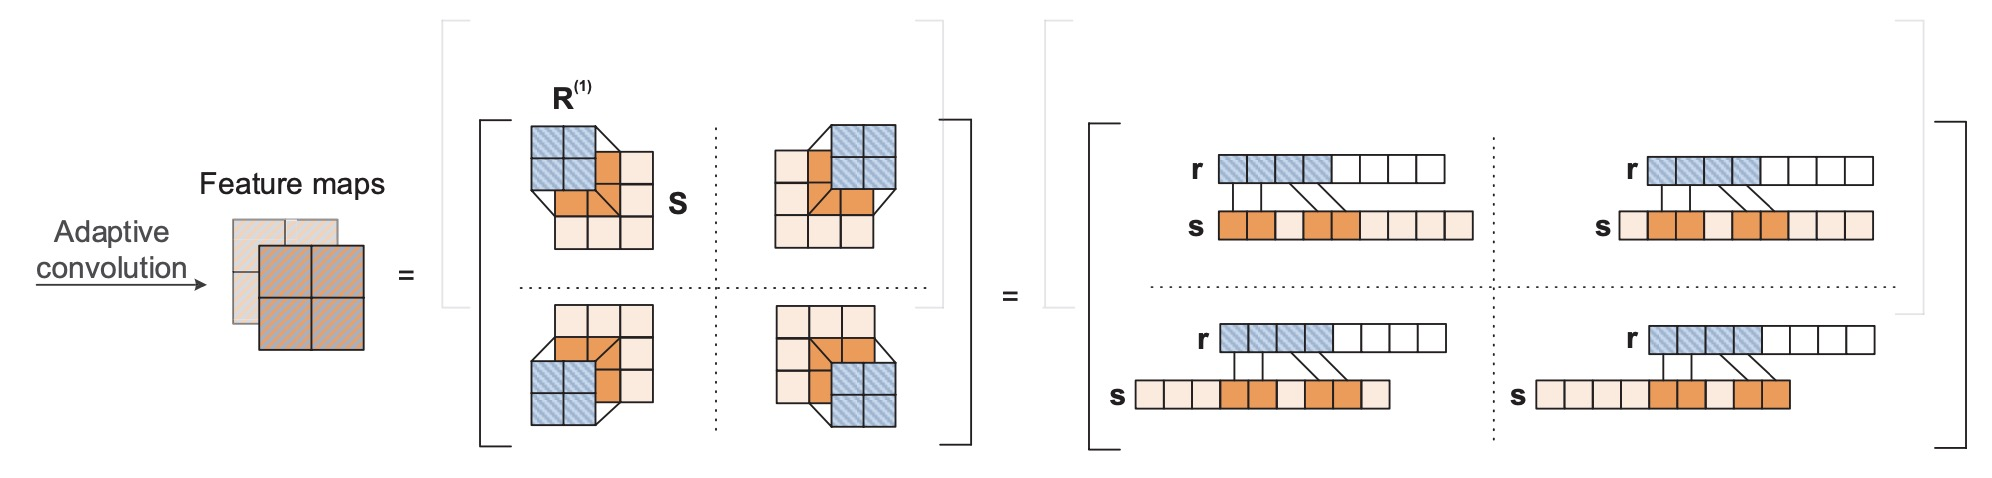
\includegraphics[width=12cm]{assets/4.png}
    \end{center}
    \item 它的本质是对两个Embedding进行元素级别的点积,即$c_{m,n}^{(l)}=f(\sum\limits_{i,j}h_{i+i-1,n+j-1}\times r_{i,j}^{(l)})$,其中$f(\cdot)$是非线性函数(作者使用的激活函数为\texttt{ReLU})。
    \item 评分函数和ConvE一致$\psi (h,r,t)=f(\mathbf{Wc+b})^{\rm T}\mathbf{t}$,其中$\mathbf{W}$和$\mathbf{b}$是用于线性变换的全连接层,$f(\cdot)$是非线性函数,损失函数也依然使用\texttt{BCELoss}。
\end{itemize}
    
\end{frame}

\subsection{实验结果与分析}

\begin{frame}[c]{Experiments}

\begin{itemize}
    \item 评分函使用$f({\rm \mathbf{Wc+b}})^{\rm T}{\rm \mathbf{t}}$,即输入的$h$和$r$元组时会计算得到关于所有尾实体的评分,并计算其中真实三元组$(h,r,t)$的Hit和MRR指标,基于WN18RR和FB15k-237进行对比实验。
\end{itemize}

\begin{center}
    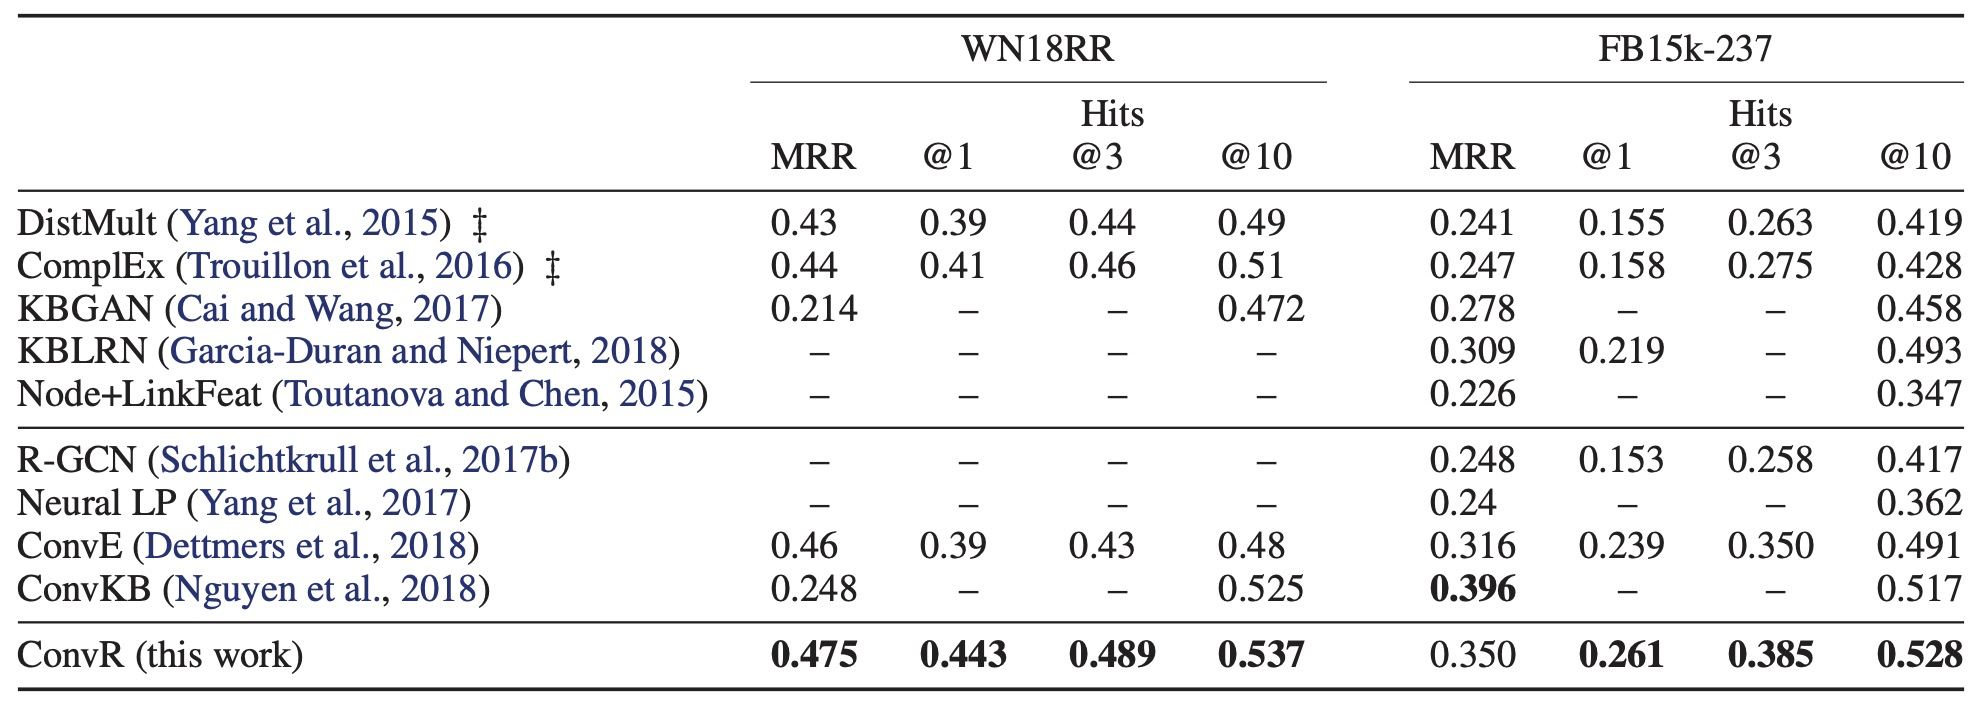
\includegraphics[width=13cm]{assets/5.png}
\end{center}

\end{frame}

\begin{frame}[c]{Hyper parameters}

\begin{itemize}
    \item 对比了不同超参数量下的实验指标(每个单元内依次为参数量、MRR、Hits@10),和ConvE相比使用了更少的参数量并达到更高的指标。
\end{itemize}

\begin{center}
    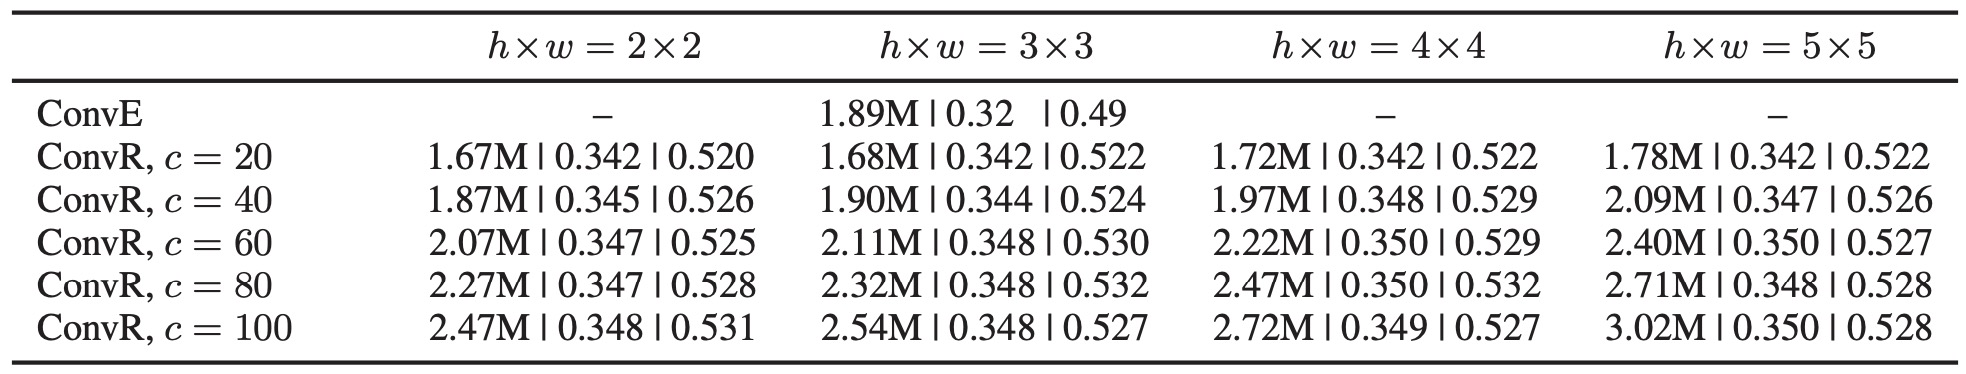
\includegraphics[width=13cm]{assets/6.png}
\end{center}

\end{frame}

